It is outside of the scope of this thesis to give an exhaustive account of classification in machine learning and as such no dedicated section to explain this is included in the theory chapter, but for good measure a brief introduction to the subject is given below. Supervised learning constitutes a very rigid analytical paradigm: given a set of \textit{observations} $\matr{X} = [\matr{x}_1, \matr{x}_2, ..., \matr{x}_n]^\top \in \mathbb{R}^{n \times m}$ which has a corresponding set of \textit{labels} $\matr{y} = [\matr{y}_1, \matr{y}_2, ..., \matr{y}_n]^\top \in \mathbb{R}^{n \times 1}$ supervised learning aims to learn the labels that typically result from different types of observations. If the labels for example were "cat" or "dog", and features were "paw size", "body weight", "has whiskers", "barks", a supervised machine learning algorithm would be trained to learn the \textit{decision boundary} that separates the classes and be able to predict whether new unseen data corresponded to a cat or a dog. Modeling is, however, not always the primary concern when applying supervised machine learning. As is the case with the current analysis, it is often desired to get an estimate of the \textit{accuracy} with which a target variable can be predicted from a given type of data. To do this, the orignal dataset $\matr{X}$ is split into a \textit{training fold} $\matr{X_\mathrm{train}}$ and a \textit{test fold} $\matr{X_\mathrm{test}}$. The model is then trained on $\matr{X_\mathrm{train}}$ and the reported accuracy is the percentage of labels it guess correctly when it is tested on $\matr{X_\mathrm{test}}$. This sectioning of training and test data can be done in a variety of ways to get the most information out of the available data. In the current analysis a \textit{cross validation} approach is used for doing this. There exist many different models for classification one of the simplest being \textit{decision trees} that learns to separate data by sequential decision rules which best separates it into different classes. An extension of this model is the \textit{random forest} which trains many trees that in turn "vote" for which class a given sample should belongs to.

Section \ref{subsec:classification} investigates whether consensus archetypes provide better prediction targets than Big Five traits and QI PCs using a supervised machine learning approach. For each target accuracy is reported for a three-class optimized random forest classifier which is validated using a random sampling cross-validation approach (explained below). The optimization scheme optimizes the parameters \texttt{n\_estimators} and \texttt{max\_features} which are generally considered the most important parameters to tune for random forest models\mcite{sklearnEnsemble}. \texttt{n\_estimators} decides the number of trees which the forest model trains and uses for voting, and \texttt{max\_features} is the maximal number of randomly selected features which are considered at each split. The scheme works in two steps: (1) estimate validation scores 100 times for random parameter settings and record the parameter combination $(p_1^{opt},p_2^{opt})$ which lead to the highest score, then (2) do a $10 \times 10$ grid-search in the quadratic range of $[p_1^{opt}-\frac{p_1^{opt}}{2}; p_1^{opt}+\frac{p_1^{opt}}{2}]$ and $[p_2^{opt}-\frac{p_2^{opt}}{2}; p_2^{opt}+\frac{p_2^{opt}}{2}]$ to find the optimal parameters.

Cross-validation is performed over 100 folds. In each fold the model is trained on a subset of 80\% randomly selected samples from the dataset and tested on the remaining 20\%. The reported accuracy is the average of this. SD of acuracies across folds are around 2\% so for 100 fold the standard error evaluates to around 0.2\%.

% \begin{figure}
% 	\centering
% 	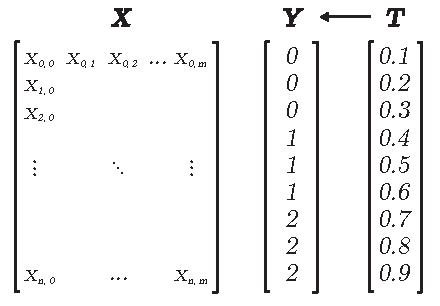
\includegraphics[width=0.5\textwidth]{figures/learningParadigm}
% 	\caption{\label{fig:learningParadigm} Example of how three classes are computed a continuous variable $\matr{T}$. $\matr{Y}$ is the vector of classes that the model learns using data-samples $\matr{X}$.}
% \end{figure}